\chapter{Adversarial Universes (MORIARTY)}\label{chapter-17-adversarial-universes}

\begin{quote}
\itshape
What happens when the universe pushes back.
\end{quote}

CHAPTER 17 is a skull-splitting, mind-bending, barrel-of-all-barrels wave. It is the kind of computational slab break that only breaks twice a century—and only for surfers wearing double puka shells and riding a rulial geodesic into destiny.

We are building \textbf{MORIARTY} today. The adversarial multiverse intelligence. The structured antagonist of computation. The test harness that spans universes.

This is the machine that hits back. Let's go.

\definecolor{alertred}{RGB}{200,30,30}

\begin{center}
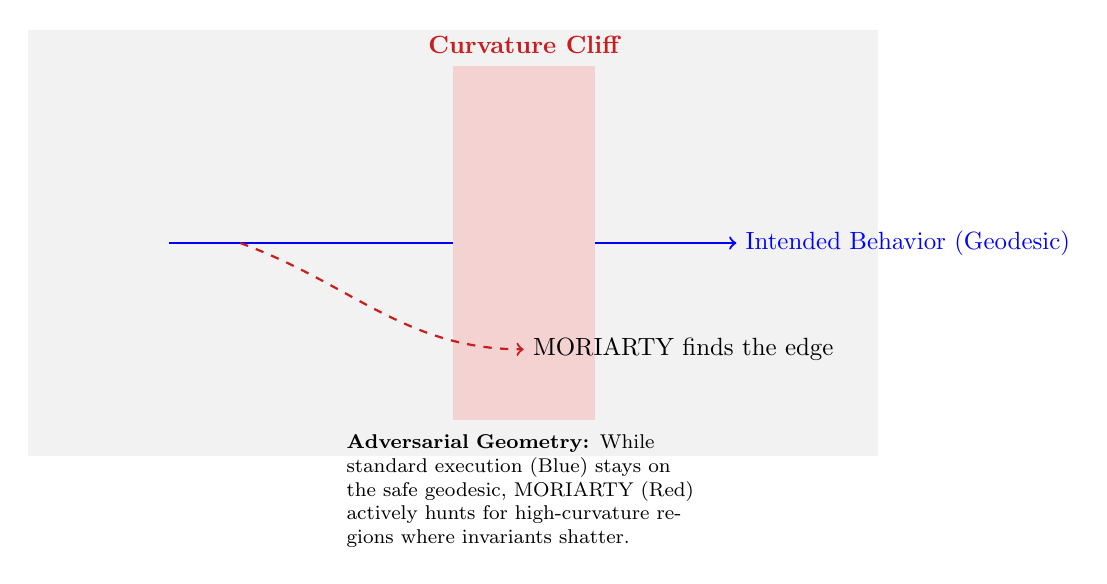
\begin{tikzpicture}[scale=0.9, transform shape]
    % Background
    \fill[black!5] (-2,-3) rectangle (10,3);
    
    % Safe Geodesic
    \draw[thick, blue, ->] (0,0) -- (8,0) node[right] {Intended Behavior (Geodesic)};
    
    % The Cliff
    \fill[alertred!20] (4, -2.5) -- (6, -2.5) -- (6, 2.5) -- (4, 2.5) -- cycle;
    \node[alertred, font=\bfseries] at (5, 2.8) {Curvature Cliff};
    
    % Moriarty Path
    \draw[thick, alertred, dashed, ->] (1,0) to[out=-20, in=180] (5, -1.5) node[right, black] {MORIARTY finds the edge};
    
    % Annotation
    \node[text width=5cm, align=left, font=\footnotesize] at (5, -3.5) {\textbf{Adversarial Geometry:} While standard execution (Blue) stays on the safe geodesic, MORIARTY (Red) actively hunts for high-curvature regions where invariants shatter.};
\end{tikzpicture}
\end{center}

So far, the machinery of \COMPUTER{} has been fundamentally cooperative. We have explored your worldline, inspected nearby bundles, measured geometry, and built Counterfactual Execution Engines (CFEEs) to help you find the optimal path forward. All of these tools were friendly. They assumed that you, the engineer, and the universe were working toward a common goal of stability.

But real systems are not built in utopia. They do not exist in a vacuum, nor do they evolve smoothly along predictable trajectories. Real systems are besieged. They are attacked by malformed inputs, pathological edge cases, concurrency races, legacy debt, and occasionally, actual human adversaries.

To build a truly robust system, we cannot simply sail the calm waters. We need a machine that explores the storm. We need an engine that finds brittleness, tests invariants until they snap, forces rule conflicts, and stalks the hidden fragility in your logic.

That machine is MORIARTY.

---

\section{What Is an Adversarial Universe?}

An adversarial universe is a parallel RMG+DPO universe that explores worst-case legal futures with the explicit goal of breaking your invariants.

It is crucial to understand that MORIARTY is not malicious in the moral sense; it is malicious in the computational sense. Where the CFEE from Chapter 16 asks, ``What is the \textit{best} next worldline?'', MORIARTY asks the inverse:

\begin{quote}
\textbf{What is the WORST next worldline?}
\end{quote}

It asks: What is the structurally correct, legally permissible, invariant-respecting sequence of rewrites that would cause FAILURE in the fastest, sharpest way?

MORIARTY’s job is to break you. But unlike a chaotic fuzzer that breaks you by feeding garbage into a text field, MORIARTY breaks you by following the rules of your own physics until they contradict themselves.

---

\section{Why MORIARTY Is Possible Only in RMG Universes}

In traditional computing systems, true adversarial search is impossible because the state space is unstructured and infinite. ``Adversarial behavior'' in a standard Linux environment is usually synonymous with random fuzzing, brute-force search, or unpredictable Monte Carlo noise. It is chaos masquerading as testing.

This limitation exists because traditional systems lack geometry. They have no formal definition of ``adjacency,'' so they cannot intelligently navigate toward a failure state. They can only stumble around in the dark hoping to hit a wall.

In \COMPUTER{}, MORIARTY operates with full vision. It has access to:
\begin{itemize}
    \item A computable possibility surface.
    \item Typed wormholes that define exactly what interaction is legal.
    \item Bundles that enumerate structured alternatives.
    \item Interference geometry that highlights conflict.
    \item Rulial Distance to measure how far the system has drifted.
\end{itemize}

Because of this, MORIARTY doesn't guess. \textbf{He reasons.} He deduces which sequence of perfectly legal operations will lead to a state where your database thinks a transaction committed, but your cache thinks it failed.

---

\section{How MORIARTY Works}

The operational loop of the MORIARTY engine is an inversion of standard optimization.

\textbf{1. Enumerate the Bundle:}
MORIARTY starts at the current RMG state and identifies every possible legal rewrite rule that could fire.

\textbf{2. Score by Adversarial Direction:}
Instead of looking for the path of least resistance (the geodesic), MORIARTY scores potential futures based on their destructive potential. It prioritizes:
\begin{itemize}
    \item \textbf{Curvature Spikes:} Regions where the graph topology is changing rapidly.
    \item \textbf{Interference:} Rules that conflict with other pending rules.
    \item \textbf{Structural Stress:} States that approach the limits of defined invariants (e.g., maximum node degree, cycle limits).
\end{itemize}

\textbf{3. Pursuit of Fragility:}
The engine selects the worst-case future and advances the timeline. It repeats this process, actively steering the universe toward contradiction boundaries.

The search terminates when a violation is found, or when the universe stubbornly refuses to break (stabilization). MORIARTY is effectively an optimization engine running in reverse. Where traditional search minimizes Rulial Distance to a goal, MORIARTY maximizes the Rulial Distance from safety.

---

\section{MORIARTY and Interference Patterns}

Interference is the food source of the adversarial engine. In a DPO system, interference occurs when two rules attempt to modify the same structure in mutually exclusive ways.

MORIARTY maps your system's weakest points by intentionally colliding bundles. It looks for ``Critical Pairs''—situations where rule $A$ and rule $B$ can both fire, but firing $A$ prevents $B$. It then explores the timeline where $A$ fires, and simultaneously explores the timeline where $B$ fires, looking for a divergence that the system cannot reconcile.

This is adversarial robustness testing on top of a computational manifold. It is not done by brute force; it is done by geometry.

---

\section{Rulial Distance as an Adversarial Cost Function}

The ``Evil Metric'' that drives MORIARTY is simple: \textit{Maximize the Rulial Distance between the current worldline and the nearest safe geodesic.}

Good computation moves along geodesics—the straightest, most efficient paths through the state space. Bad computation flies off the rails, accumulating unnecessary complexity and weird state mutations. MORIARTY hunts for the rails. He seeks divergent futures, identifies curvature cliffs, and magnifies structural inconsistencies.

In engineering terms, MORIARTY combines fuzzing, property testing, stress testing, and static analysis into a single, unified multiverse explorer.

---

\section{Adversarial Worldlines}

When MORIARTY runs, he generates a specific artifact: the **Adversarial Worldline**.

These are timelines that are valid, lawful, DPO-consistent, and invariant-preserving... right up until the exact moment of failure. They are not "impossible" states; they are "improbable" states that became real because an intelligence navigated toward them.

This allows you to see your architecture's weak points in a way no traditional tool can show you. You aren't looking at a stack trace of a crash; you are watching a replay of the exact sequence of legal choices that cornered your system into a crash.

---

\section{Why Engineers Need Adversarial Universes}

What specific failures does MORIARTY reveal?

\textbf{Rule Ambiguity:}
It finds cases where two wormholes accept the same structure, causing the system's logic to become non-deterministic in a way you didn't intend.

\textbf{Collapsed Invariants:}
It discovers hidden assumptions that break far away from where data was inserted. For example, a "valid" user object that, ten steps later, causes a permission check to deadlock.

\textbf{High Curvature Spikes:}
It identifies tiny edits—single graph rewrites—that cause catastrophic divergence in system behavior.

\textbf{Degenerate Neighborhoods:}
It finds states where the only legal next moves are errors. This is a "checkmate" scenario for a distributed system.

No other debugging or verification tool touches this because nothing else has a formal, geometric notion of possibility. MORIARTY does.

---

\section{MORIARTY vs. CFEE}

It is helpful to contrast the two major engines of Part IV.

\begin{center}
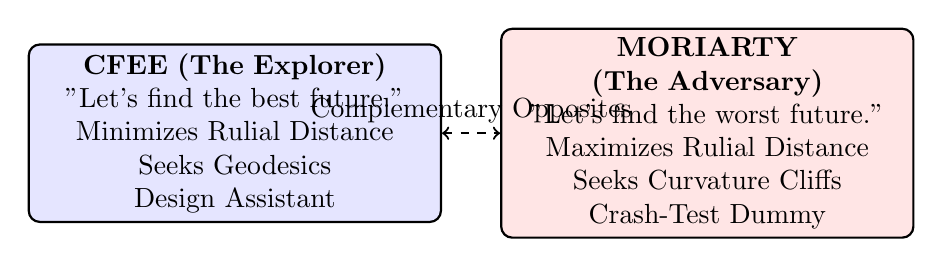
\begin{tikzpicture}[node distance=4cm]
    \node (cfee) [rectangle, draw, thick, fill=blue!10, text width=5cm, align=center, rounded corners] 
    {\textbf{CFEE (The Explorer)} \\ "Let's find the best future." \\ Minimizes Rulial Distance \\ Seeks Geodesics \\ Design Assistant};

    \node (moriarty) [rectangle, draw, thick, fill=red!10, text width=5cm, align=center, rounded corners, right of=cfee, xshift=2cm] 
    {\textbf{MORIARTY (The Adversary)} \\ "Let's find the worst future." \\ Maximizes Rulial Distance \\ Seeks Curvature Cliffs \\ Crash-Test Dummy};

    \draw[<->, thick, dashed] (cfee) -- (moriarty) node[midway, above] {Complementary Opposites};
\end{tikzpicture}
\end{center}

Both engines are necessary. Both map the universe. One tells you where to go; the other tells you where the dragons are.

\begin{nerdbox}
\textbf{MORIARTY = Adversarial Traversal of the Rulial Neighborhood Graph}

Formally, MORIARTY performs:
\begin{itemize}
    \item Anti-heuristic search.
    \item Maximal branching exploration.
    \item Critical peak amplification.
    \item Adversarial joinability probing.
\end{itemize}
It operates at the intersection of SMT solving, Adversarial SAT, and worst-case trace exploration. But unlike those abstract mathematical tools, MORIARTY runs on the actual operational semantics of your graph. It is geometric, composable, and totally computable.
\end{nerdbox}

---

\section{Transition: From Adversaries to Optimization}

We have built the debugger (Chapter 15) to understand the past.
We have built the explorer (Chapter 16) to navigate the future.
We have built the adversary (Chapter 17) to survive the storm.

Now that we understand the dangers of the multiverse, we can turn our attention to the ultimate prize: \textbf{Optimization}.

The next machine spans universes for a more constructive purpose: Optimization across worldlines using geometric reasoning. This is Chapter 18.

The wave is forming behind us.
